\pagenumbering{arabic}

\chapter{Images and Videos}

\section{Definitions}
\subsection{Computer Vision}
Is the science and technology of machines that see, where“see” in this case means that the machine is able to extract information from an image that is necessary to solve some task. The image data can take many forms, such as video sequences, views from multiple cameras, or multidimensional data from a medical scanner.

Some examples of applications of computer vision include systems for controlling processes, like an industrial robot or an autonomous vehicle, detecting events as for visual surveillance or people counting, or again organizing information for example for indexing databases of images and image sequences, even modeling objects or environments like in industrial inspection, medical image analysis or topographical modeling and interaction as the input to a device for computer-human interaction.

\begin{figure}[h]
    \centering
    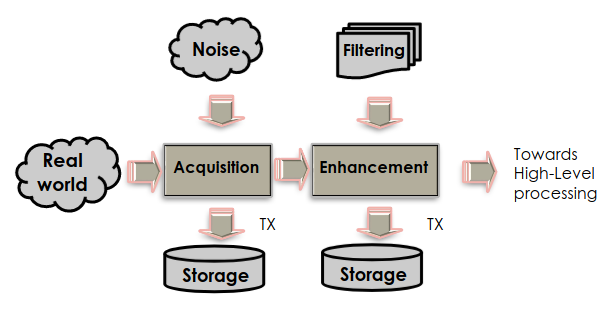
\includegraphics[scale=0.5]{Figures/ProcessingChain.png}
    \caption{The processing chain(The first part is more about signal and video, in this course we'll focus mainly on the second half)}
    \label{fig:enter-label}
\end{figure}

\subsection{Acquisition}
It refers to the process of transferring a portion of the real 3D world onto a 2D surface bringing a continuous-parameter real world into a discrete-parameter one. 
The acquisition process is the first step in the processing chain and it is the transformation of a physical signal into an electrical one, by means of a sensor. 
Where the sensor is a device that responds to a physical stimulus (light, heat, pressure, etc.) and produces an electrical signal. 
\textit{PS: The representation is in a standard format.}
\\
\subsection{Digital Images}
A digital image is a representation of a two-dimensional image as a finite set of digital values, called picture elements or pixels. 
The digital image contains a fixed number of rows and columns of pixels and so is a collection of coordinates. Pixels are the smallest individual element in an image, a single pixel represent a projection of a portion of the real world, holding quantized values that represent the brightness of a given color at any specific point. Pixels can be \textbf{Grayscale} or \textbf{Color}. 
Grayscale images are represented by a single component, typically 8bit, while color images are represented by three components, typically 24bits.
\\
\subsection{Sampling}
Is the process of converting a continuous signal into a discrete signal. This is because the "real world" is a continuous function, and computers are digital. Analog video is a 1-D continuous function where one spatial dimension is mapped onto time by means of a scanning process, while digital video is instead sampled in a three dimensions (2D spatial and 1D temporal).
\\
\begin{figure}[h]
    \centering
    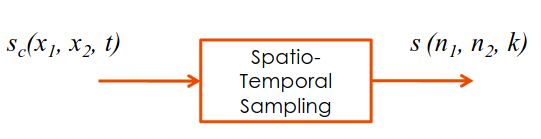
\includegraphics[scale=0.5]{Figures/Sampling.png}
    \caption{Sampling}
    \label{fig:enter-label}
\end{figure}

\textit{In a Nutshell:}
\begin{itemize}
    \item Continuous signal \[ s_c(x_1, x_2)\]
    \item Spatial rectangular sampling \[ x_1 = n_1 \bigtriangleup x_1, x_2 = n_2 \bigtriangleup x_2\]
    \item So \[ s(n_1, n_2) = s_c(n_1 \bigtriangleup x_1, n_2 \bigtriangleup x_2)\]
    \item Once we have the digital format, we can manipulate data and apply filters, change colors, store and transmit.
\end{itemize}

For what concerns handling images we need only to know that pixels are numbered starting from the top left corner (so the top left corner is the origin, arrow down for the rows and right for the columns).
The value of a pixel in a certain position is defined as \(I(r,c)\), where \(r\) is the row index and \(c\) the column one. (Start at 0 or 1, depends on you :D)
Monochrome images have values normalized in the range \([0,1]\), where 0 is black, 1 is white and the intensity is called \textit{grey level}. While color pictures have 3 channels (RGB) and the values are normalized in the same way.
\section{Color}
But what is color? It's the attribute the human visual system associates to objects, more scientifically it's a mathematical relationship that combines different wavelengths. 
It's important to check whether something we see is what we expect, to recognize objects or to distinguish similar things. For example, a white car, that for us is obviously white, for a computer is a combination of red, green and blue, moreover it has some black points for the wires, some point gray due to the street, etc.
For this reason let's talk about color perception. The human eye is like a camera with a focal length of about 20mm, where the iris controls the amount of light by adjusting the size of the pupil. 
The perception of color is possible through cones in the fovea that has around 100M receptors.  Cones have peak responses on three main wavelengths, red (700nm), green (546.1nm) and blue (435.8nm).
\\
But going back to the main topic, data can be processed locally but even transmitted remotely or archived on a storage unit. The problem is that images and videos require a lot of bandwidth, so we need to compress them with a codec.
A codec is a device or computer program for encoding or decoding a digital data stream or signal in the compressed domain. It stands for coder-decoder, and it's a way to reduce the dimension of the file (e.g JPEG, MPEG, DIVX). 
\\\textit{NB: Compression is lossy, so reduces quality (we lose some information) and can even introduces visual artifacts (such as blocking, blurring, chromatic aberrations(plus some noise from the sensor)). However, the loss is not a problem because the human visual system is not perfect.
NB1: Exist even lossless compression, but it's not used much.
NB2: Processing is typically done in the uncompressed domain. 
NB3: Raw images are vector of pixels.
}
\subsection{Additive color model}
The additive color model is a method to create color by mixing the primary colors.
\begin{figure}[h]
    \centering
    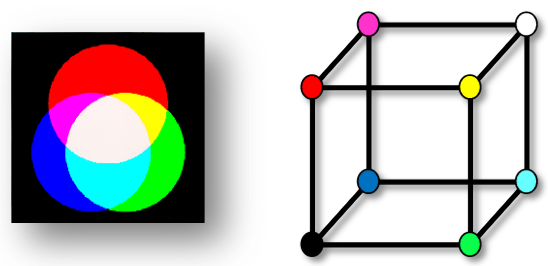
\includegraphics[scale=0.5]{Figures/AdditiveModel.png}
    \caption{Additive Color Model}
    \label{fig:enter-label}
\end{figure}

Colored beams are projected onto a black surface, then overlap so the human eye receives the stimula without generating interference, mixing the components and perceiving the resulting color.
Starting from the primary colors RGB we can obtain:
\begin{itemize}
    \item R+G = Yellow
    \item R+B = Magenta
    \item B+G = Cyan
    \item R+G+B = White
\end{itemize}
\textit{NB:Subtractive color is the inverse process.}\\
About the way colors combined, we can have:
\begin{itemize}
    \item Black: RGB(0,0,0)
    \item Green: RGB(0,1,0)
    \item Yellow: RGB(1,1,0)
    \item White: RGB(1,1,1)
    \item Gray: RGB(0.5,0.5,0.5)
\end{itemize}

Indeed, looking at the image above we can identify the gray scale along the diagonal connecting the black corner with the white corner.

\textit{NB: If we separate the three components and generate single images we notice that components are correlated, this means that the three version in grey-scale of the starting image carry almost the same amount of information.}

In RGB we have a major response in the green component, while red and blue are less relevant. In addition, human eye is more sensitive to luminance and contrast variations than color so maybe a different representation would be more effective.
Indeed, more effective is the YCbCr color space, where Y, the luminance is separated from Cb and Cr that are the chrominance.
\textit{PS: YCbCr is a generalization of YUV, just a matter of conversion matrices. (TODO: Downsampling)}
\\
Another color space is the HSV, where H is the hue (color), S is the saturation (brightness) and V is the value (intensity).

\begin{figure}[h]
    \begin{subfigure}{0.5\textwidth}
        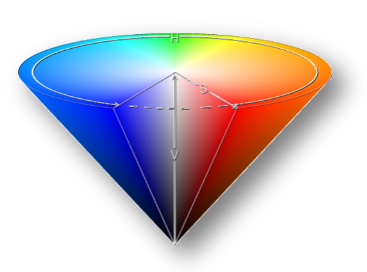
\includegraphics[scale=0.4]{Figures/HSV1.png} 
        \label{fig:subim1}
    \end{subfigure}
    \begin{subfigure}{0.5\textwidth}
        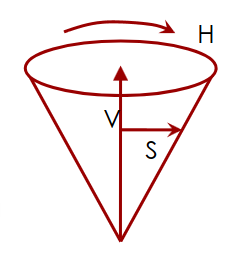
\includegraphics[scale=0.5]{Figures/HSV2.png}
        \label{fig:subim2}
    \end{subfigure}
        
        \caption{HSV Color Space}
        \label{fig:image2}
\end{figure}

Summing up just a little bit:
\begin{itemize}
    \item RGB is used in general for visualization, in displays each pixel in composed by three phosphors (CRT) or LEDs (LCD);
    \item YUV is suitable for compression since we are less sensitive to chrominance variations and U and V can be downsampled;
    \item HSV is robust for computer graphics and image analysis.
\end{itemize}

\subsection{Bayer Pattern}
In the acquisition phase, light is captured by the CCD (Charge Coupled Device) that is an array of cells. Each cell is a photosensitive element that converts light into an electrical signal.
The Bayer pattern is a color filter array for arranging RGB color filters on a square grid of photosensors. The best solution would be to have devices with 3 different CCDs and to correctly exploit the human eye response there would be three types of photosensors of color filters 50\% green, 25\% red and 25\% blue.
\textit{NB: Green sensors are defined as luminance-sensitive elements, while the red and blue ones are defined as chrominance-sensitive.}
\subsection{Quantization}
Like in the mono-dimensional case, signals need to be quantized. That implies the definition of a number of levels to define our signal. Typically, the range 0-1 is quantized using 8bpp but even other representations with 10-12 bpp are available.
But why 8bpp? well, 8bpp represent 256 levels, which is fine for the human eye, that can distinguish 100 levels of grey. Indeed, if we quantize with less that 6bpp (64 levels, minimum to ensure smooth pictures), then false contours will appear $\Rightarrow$ contouring.
\\
\subsection{Limits of the 2D}
Still images provide a reliable information about static scenes.
We lose motion information like temporal evolution of the scene, rapid changes, dynamics of motion (qualitative and quantitative) and even how subjects/objects relate one to each other.
Moreover, analyzing a video provides a more consistent representation of the scene.
It’s closer to what humans do every day.

\subsection{Video}
A video is a sequence of 2D images that represent a projection of moving 3D scene onto the video camera image plane. PS: It's expected that adjacent frames are strongly correlated.
For what concerns the resolution, the images are up to 50mp, while in video is typically lower, 4k is 3840x2160=8.3mp, 8k is 7680x4320=33.2mp and full HD is around 2mp.
The reasons are that video can last hours, so we need to store a lot of data, and the human eye is less sensitive to resolution in motion. 
Just move on a little bit, once the image is acquired, what are the most relevant features we could be interested in? Maybe color and its distribution or presence of edges and contours\dots
And again, if the analysis concerns a video, instead of an image, what is the added value?
Consistency of the features over time, evolution of the scene and objects displacement and, of course, objects that may enter or exit the scene.
\\So in the end, what makes a scene complex to analyze and process?
The presence of multiple objects, occlusions, shadows, noise, motion, illumination changes, clutter and non-rigid objects.
    TODO: vedi se aggiungere gli esempi.

\subsection{Histogram}
The histogram is a simple way to describe the color distribution of a picture, indeed, it can be seen as a probability density function and it represents the occurrence of all colors on a graph.
In other words it’s a statistical representation of the pixel values. For an MxN image
\[
    hist(p) = \frac{I(x,y)}{MxN}
\]
Where $I(x,y)$ is the intensity of the pixel at position (x,y) and $MxN$ is the total number of pixels in the image.\\
The equation holds for one component, so in case of more components, a histogram can be obtained from each of them.
\begin{figure}[h]
    \centering
    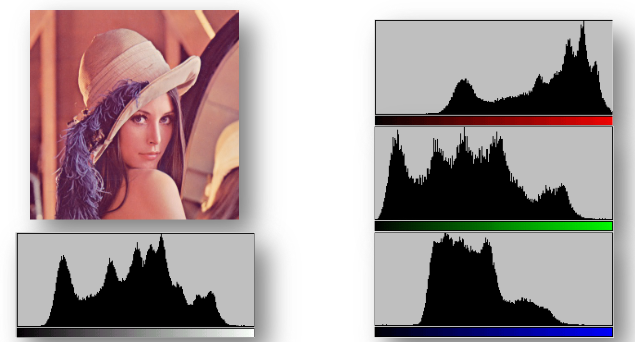
\includegraphics[scale=0.5]{Figures/Histogram.png}
    \caption{Histograms of Lana}
    \label{fig:enter-label}
\end{figure}
So, what kind of information can we obtain from the histogram?
    \begin{itemize}
        \item Is the image dark or bright?
        \item Are colors distributed equally?
        \item Are there dominant colors?
        \item Are there colors missing?
    \end{itemize}
    
    Some applications:
    \begin{itemize}
        \item Is the illumination of a scene correct for environmental monitoring?
        \item How has the background changed in the past 2 hours?
        \item Can I use the histogram to determine whether the moving object I’m observing is A or B?
    \end{itemize} 
    
    In general it can be seen as a “signature” to be applied in different domains.
    
\subsection{Operations}

\textbf{Stretching:}
\\A simple operation to change the dynamic range of the image by stretching the histogram and increasing the contrast. Usually apply a piecewise linear function. 
\begin{figure}[h]
    \centering
    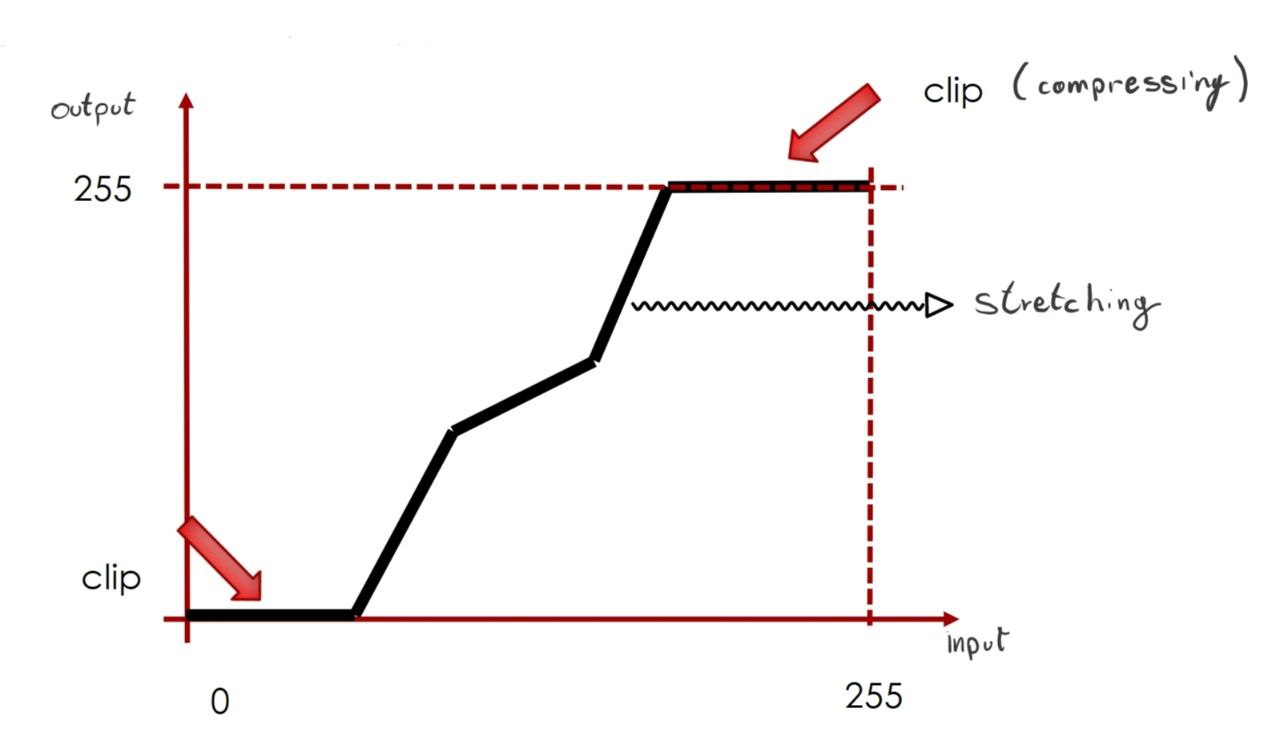
\includegraphics[scale=0.3]{Figures/Stretching.jpeg}
    \caption{Stretching}
    \label{fig:enter-label}
\end{figure}   
\\ 
\textbf{Equalization:}
\\Working on the statistics of the pixels it is possible to improve the quality of an image. Ideally we’d like to obtain a FLAT histogram, and to do so we have to compute the cumulative histogram (equivalent to CDF).
    \[
        CHist_I(p) = \sum_{k=0}^{p} hist(k)
    \]
    \[
        hist_eq(p) = \frac{CHist(p)-CHist_{min}}{M \times N-1}\times 255
    \]
\begin{figure}[h]
    \centering
    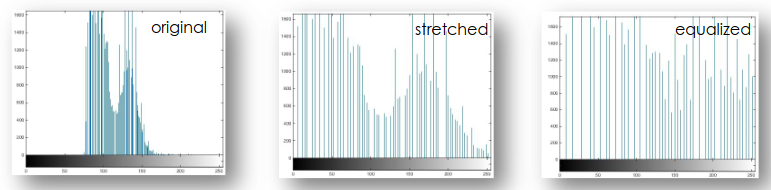
\includegraphics[scale=0.5]{Figures/OperationsHist.png}
    \caption{Different operations on the histogram}
    \label{fig:enter-label}
\end{figure}
    
\section{Edge extraction}
We perceive objects through color (appearance model) and shape. Shape is the boundary between the object and the rest of the picture, and it helps us recognizing things.
A sharp change in image brightness can be seen as an edge.
\\PS: Environmental conditions, such as cast shadows or surface orientation, can generate changes. Moreover edges are not always meaningful, for example in textured areas or in the presence of noise.
\\Steps:
\begin{itemize}
    \item Determine intensity, and possibly the direction of an edge for each pixel location through gradient or Laplacian;
    \item Find a threshold and binarize.
\end{itemize}
\textit{NB: The first step is the most difficult one. Different tools are available but we’ll focus here on the gradient-based algorithms.}
\\
\textbf{Edge extraction by gradient analysis}\\
As for mono-dimensional signals, the goal is to find maxima and minima but in this case, we also have a direction. This means finding a gradient along a line $r$ oriented in the direction $\theta$.
\[
\frac{\partial f}{\partial r} = \frac{\partial f}{\partial x}\frac{\partial x}{\partial r} + \frac{\partial f}{\partial y} \frac{\partial y}{\partial r} = f_x \cos(\theta) + f_y \sin(\theta)
\]
\\
The edge extraction process consists of computing the 1st order derivative in two orthogonal directions, $f_1$ and $f_2$. To each of them we associate an amplitude.
Going a little more into the concrete, for edge detection typically we use FIR filters, that are linear and shift-invariant. The most common are the Prewitt, Roberts and Sobel operators.
\\
For the first two we have to choose a convolution mask and apply it to the picture. The convolution is computed for both masks and a threshold is chosen to highlight only the strongest edges.
\\
\textbf{Roberts operator:} $\begin{bmatrix} 1 & 0 \\ 0 & -1 \end{bmatrix} \quad \begin{bmatrix} 0 & 1 \\ -1 & 0 \end{bmatrix}$
\vspace{0.5cm} 
\textbf{Prewitt operator:} $\begin{bmatrix} -1 & 0 & 1 \\ -1 & 0 & 1 \\ -1 & 0 & 1 \end{bmatrix} \quad \begin{bmatrix} -1 & -1 & -1 \\ 0 & 0 & 0 \\ 1 & 1 & 1 \end{bmatrix}$
\\
\textit{NB: The Prewitt operator is preferred because it is isotropic $\Rightarrow$ you know where is the center.}
\\
For the Sobel operator, we have to apply two masks, one for each orthogonal direction. The mask is a 3x3 matrix and the gradient is computed for each point. Then we have to threshold the result.
\\\vspace{1cm} 
\textbf{Sobel operator:} $D_x=\begin{bmatrix} -1 & 0 & 1 \\ -2 & 0 & 2 \\ -1 & 0 & 1 \end{bmatrix} \quad D_y=\begin{bmatrix} -1 & -2 & -1 \\ 0 & 0 & 0 \\ 1 & 2 & 1 \end{bmatrix}$
\\
The convolution with the FIR masks is performed similarly to the 1D convolution. Take the mask, rotate, slide from left to right and associate to the central point the value of the convolution. (formule ancora da mettere, non avevo voglia sorry)
\begin{figure}[h]
    \centering
    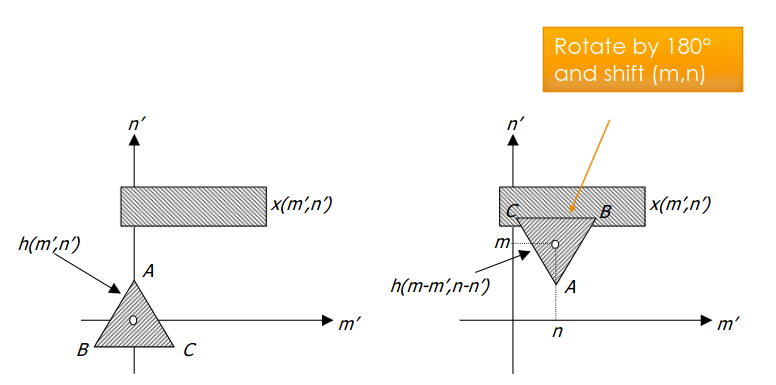
\includegraphics[scale=0.3]{Figures/Convolution.png}
    \caption{How to (convolution edition)}
    \label{fig:enter-label}
\end{figure}

\section{Filters}
\subsection{Low-pass filtering}
The easiest way is to average the values in the sliding window. The window is a matrix of size $m \times n$ and the result is the average of the values in the window.
\[
    I_{LP}(x,y) = \frac{1}{mn} \sum_{x=-a}^{a} \sum_{y=-b}^{b} I(x,y)
\]
Preserve low-frequency components and remove high-frequency ones. It's a weighted sum of low high frequency functions. Cut the high frequency components above the threshold and smooth the image. Average filtering $\Rightarrow$ average of the pixels in the window. Bigger the filter, more the smoothing (the difference is smaller). It helps denoising the signal.

\subsection{Gaussian filtering}
Gaussian filtering is a low-pass filter that is used to remove the high-frequency components of the image. It is a 2D convolution filter that is used to blur the image and remove noise. 
Gaussian try to reconstruct a gaussian function, so it's isotropic and the mask is not flipped. The mask is a 2D Gaussian usually centered in the center of the filter mask, set big enough to make sure values in the mask are integer. Using a Gaussian as a mask is convenient as in the Fourier domain it is still a Gaussian, it is isotropic (simmetric) and no need to flip the mask (no rotation in convolution).
\[
    G(x,y) = \frac{1}{2\pi\sigma^2}e^{-\frac{x^2+y^2}{2\sigma^2}}
\]
the bigger the better. The central pixels are more considered, far pixels have a lower impact.
\subsection{Median filtering}
\begin{figure}[h]
    \centering
    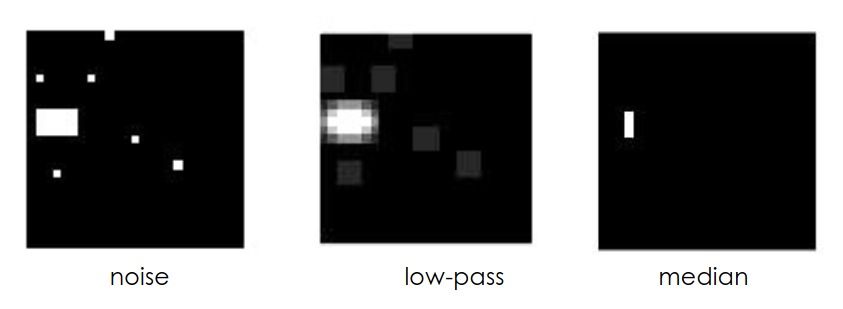
\includegraphics[scale=0.5]{Figures/Noise.png}
    \label{fig:enter-label}
\end{figure}
Median filtering is a nonlinear method used to remove noise from an image. It is a spatial domain method that replaces the pixel value with the median value of the neighborhood pixels. It is particularly effective in removing salt and pepper noise. It is a good method to use when the image is corrupted by impulse noise. 
In case the noise is zero-mean, smoothing is fine. But when you have spikes, LP filtering blurs also the noise.
Indeed, LP spread the dot, so it generates artifact. The noise is less visible but larger. Median avoid this issue, remove noise, no linear function, no convolution, sorting operation for every shift, filter ranks the values of the filter from bigger to smaller and store the median value in the central pixel. Bigger could introduce artifacts, so it's better to use a small filter. The noise that remains is because the size of the mask is not big enough to cover the noise.
\section{Morphology}
Morphology refers to the shape of a region. The goal is to check whether a certain shape fits into another, check whether a picture has holes of a certain size, remove areas smaller than a threshold and with certain shape, etc. 
\textit{PS:It refers to non-linear filtering.}
It uses a structuring element, a known arbitrary shape, and the operations are performed by sliding the structuring element over the image. The structuring element has an origin (typically central point, but not necessarily) and the operation is performed by comparing the structuring element with the image.
There are four main operations: Erosion, Dilation, Opening and Closing.\\
Erosion and Dilation are self-explanatory, the first one reduces the area of a shape, the second one enlarges it. Instead, opening and closing are a combination of erosion and dilation. Opening gets rid of small portions of the image close to the boundaries of relevant areas, while closing fills holes and makes region boundaries smoother. 
\textit{Concerning structuring elements, depending on the type of shape we want to edit, the right element must be chosen.}
\subsection{Dilation}
Dilation is a morphological operation that is used to enlarge the boundaries of regions of foreground pixels in an image. It is used to merge the objects in the image. The structuring element is a binary mask that defines the neighborhood of the pixel. The dilation of the image is obtained by sliding the structuring element over the image and placing the origin of the structuring element at the center of the pixel. 
More formally, the dilation of an image $B$ by a structuring element $S$ is given by:
\[
    B \oplus S = \cup_{b \in B} S_b
\]
Sweep the structuring element on the whole image, as the origin of the structuring element touches a “1” of the image all pixels of the structuring element are OR’ed to the output image. 
\textit{PS: OR/union $\Rightarrow$ every time that the structuring element touches a 1, the output is 1, so it enlarges the shape.}
\begin{figure}[h]
    \centering
    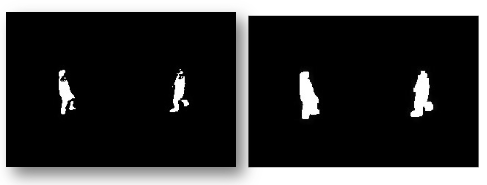
\includegraphics[scale=0.5]{Figures/Dilatation.png}
    \caption{Dilation}
    \label{fig:enter-label}
\end{figure}
\subsection{Erosion}
Erosion is a morphological operation that is used to reduce the boundaries of regions of foreground pixels in an image. It is used to separate the objects in an image.
Sweep the structuring element on the whole image, at each position where every 1-pixel of the structuring element covers a 1-pixel of the binary image the binary image corresponding to the origin is OR’ed with the output image. 
More formally, the erosion of an image $B$ by a structuring element $S$ is given by:
\[
    B \ominus S = \{b | b + S \in B \quad \forall s \in S\} 
\]
Erosion of A by B can be understood as the locus of points reached by the center of B when B moves inside A.
\begin{figure}[h]
    \centering
    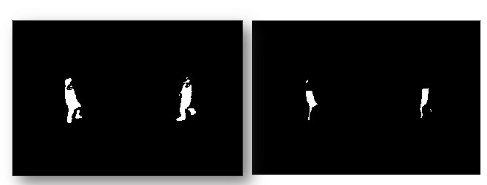
\includegraphics[scale=0.5]{Figures/Erosion.png}
    \caption{Erosion}
    \label{fig:enter-label}
\end{figure}
\\
\textit{PS: se prima bastava che il centro toccasse un 1, ora TUTTI devono toccare un 1.}
\subsection{Closing and Opening}
\begin{itemize}
    \item Closing $\Rightarrow$ first dilatate and then erode; \\Non-contiguous regions are firs merged, then the boundaries are refined.
    \item Opening $\Rightarrow$ first erode and then dilatate; \\First small areas are removed, then residual information is refined.
\end{itemize}
\begin{figure}[h]
    \begin{subfigure}{0.5\textwidth}
        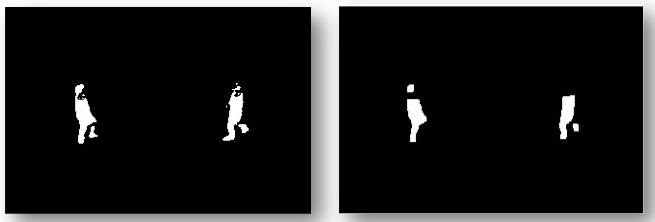
\includegraphics[scale=0.4]{Figures/Opening.png} 
        \caption{Opening}
        \label{fig:subim1}
    \end{subfigure}
    \begin{subfigure}{0.5\textwidth}
        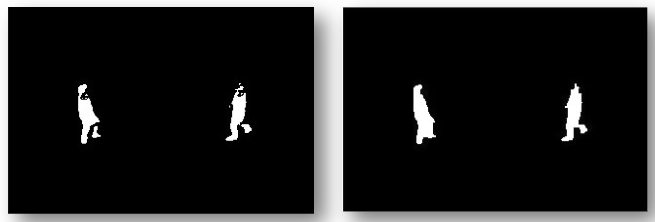
\includegraphics[scale=0.4]{Figures/Closing.png}
        \caption{Closing}
        \label{fig:subim2}
    \end{subfigure}
        \label{fig:image2}
\end{figure}
This operations are in general non-reversible, so the result depends on the order of the operations.
